\documentclass{article} % For LaTeX2e
\usepackage{nips15submit_e,times}
\usepackage[colorlinks,linkcolor=red]{hyperref}
\usepackage{url}
\usepackage{amsmath}
\usepackage{graphicx}
\usepackage{float}
\usepackage{bm}
\usepackage{amssymb}
%\documentstyle[nips14submit_09,times,art10]{article} % For LaTeX 2.09


\title{CS499 Homework 6 (First Draft)}


\author{
	Intersteller\thanks{ Use footnote for providing further information
		about author (webpage, alternative address)---\emph{not} for acknowledging
		funding agencies.}
	Department of Computer Science
	Cranberry-Lemon University
	Pittsburgh, PA 15213
}

% The \author macro works with any number of authors. There are two commands
% used to separate the names and addresses of multiple authors: \And and \AND.
%
% Using \And between authors leaves it to \LaTeX{} to determine where to break
% the lines. Using \AND forces a linebreak at that point. So, if \LaTeX{}
% puts 3 of 4 authors names on the first line, and the last on the second
% line, try using \AND instead of \And before the third author name.

\newcommand{\fix}{\marginpar{FIX}}
\newcommand{\new}{\marginpar{NEW}}

%\nipsfinalcopy % Uncomment for camera-ready version

\begin{document}

	\maketitle
	\textbf{Exercise 6.1}\par

    $(1)$As the picture shows:\par
    \begin{figure}[H]
		\centering
		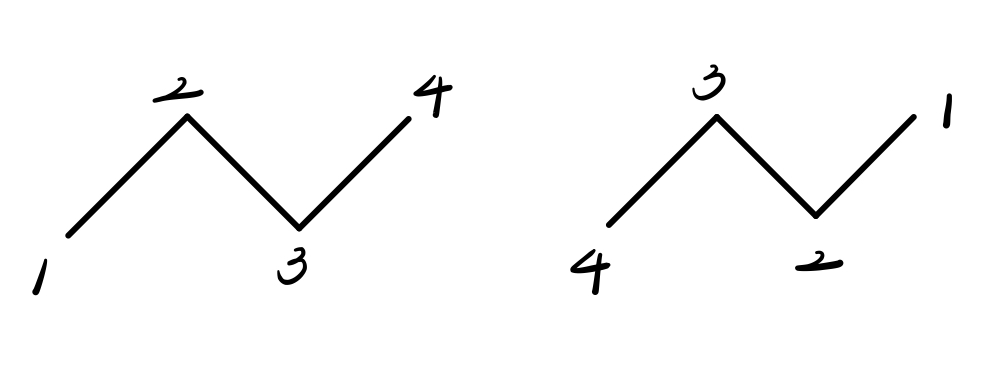
\includegraphics[scale=0.3]{p31.jpg}
		\caption{}
		\label{fig:1}
	\end{figure}
	The number of automorphisms is 2.
    $(2)$Suppose the original picture is\par
    \begin{figure}[H]
		\centering
		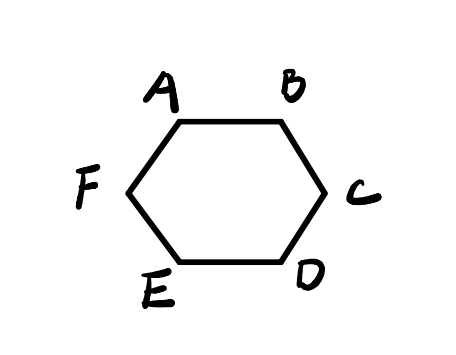
\includegraphics[scale=0.4]{p32.jpg}
		\caption{}
		\label{fig:2}
	\end{figure}
    Original $A$ position now is $A'$,so original $B$ position now is the point connected with $A'$ before and there are two possibilities.\par
    If $B'$ is determined,the original $F$ position is the other point connected with $A'$ apart from $B'$.\par
    Therefore other positions is also determined for the same reason, as in the following figure.\par
    \begin{figure}[H]
		\centering
		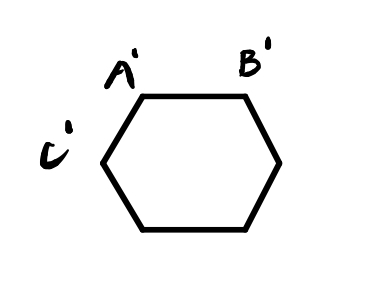
\includegraphics[scale=0.4]{p33.jpg}
		\caption{}
		\label{fig:3}
	\end{figure}
    So the number of automorphisms is $6 \times 2 = 12.$\par
    $(3)$For the same reason of $(2)$,if there are 3 points  determined , the graph is determined.\par
    So the number of automorphisms is $8 \times 3! = 48$.

	
	

	\textbf{Exercise 6.2}\par
    The complete graph on $999$ vertices has $C_{999}^{2}$ edges.The $|E|$ is odd,so the $|E|$ of original graph and the $|E|$ of complement graph is not equal.
    So there is no self-complementary graph on $999$ vertices.

	\textbf{Exercise 6.3}\par
	\textbf{Theorem:}  There is a self-complementary graph on $n$ vertices if and only if $n=4k$ or $n=4k+1$. (here and in the following, $k=1,2,3,\cdots$)\par
	\textbf{proof:}\\
	(1)  If $n=4k+2$ or $n=4k+3$, since a complete graph has $\frac{(|V|-1)(|V|-2)}{2}$ edges, $|E|$ will be an odd number. It is obvious that if $|E|$ is an odd number, the graph can not be self-complementary.\par
	(2)  If $n=4k$, we can show the graph is self-complementary in the following method:\\
	We divide the vertices into 4 sequences A, B, C and D, each sequence has k verticies. Then we add $\frac{(k-1)(k-2)}{2}$ edges into sequence A and sequence B respectively.After that we add $\frac{(k)(k-1)}{2}$ edges between sequence A and sequence B, sequence A and C, sequence B and sequence D respectively, as in the following figure. 
	\begin{figure}[H]
		\centering
		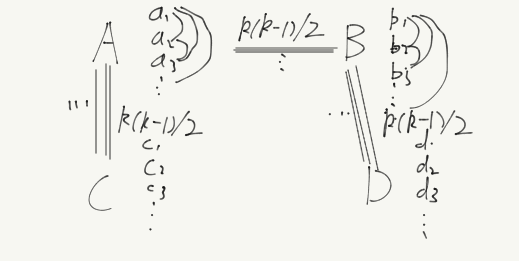
\includegraphics[scale=0.8]{p1.png}
		\caption{}
		\label{fig:4}
	\end{figure}

	In this way we get a graph G, whose complementary graph is G', which has $\frac{(k-1)(k-2)}{2}$ edges in sequence C and in sequence D respectively, and $\frac{(k)(k-1)}{2}$ edges between sequence A and sequence D, sequence B and sequence C, sequence C and sequence D respectively. Through the bijection $C\rightarrow A$ ($c_1\rightarrow a_1, c_2\rightarrow a_2,\cdots$ (and the same in the following)), $A\rightarrow D$, $B\rightarrow C$ and $D\rightarrow B$, we can show that G and G' are automorphism, which means G or G' is a self-complementary graph.\par
	(3)  If $n=4k+1$, we divide the vertices into 4 sequences same as above and 1 special dot. Then for the sequences we use the same method to add edges, except in graph G we add k edges between A and the dot, B and the dot respectively. Then we will have k edges between C and the dot, D and the dot respectively in G'. In the bijection we add $dot \rightarrow dot$. In this way, G or G' is still self-complementary graph.


	\textbf{Exercise 6.4}\par
	For $k=3$ and $k=4$, the corresponding graphs are in the following figure.
	\begin{figure}[H]
		\centering
		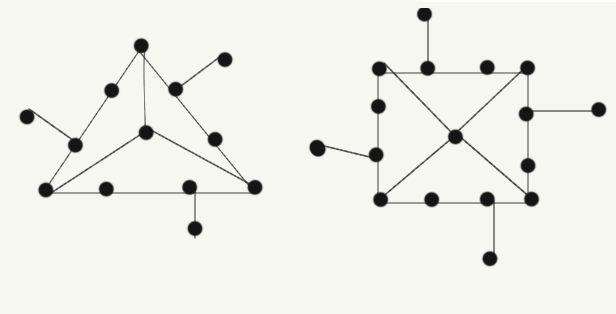
\includegraphics[scale=0.8]{p2.png}
		\caption{}
		\label{fig:5}
	\end{figure}
	\textbf{One general construction method:} For $k=n$, first we draw a polygon that has n edges. Then we add one vertex in the middle of the polygon and link it with n vertices respectively. After that we add 2 verticies on each edge. Finally, we add one vertex and one edge in every 3 vertices clockwise. 

	\textbf{Exercise 6.5}\par
	For every $n\le6$, there is an asymmetric graph on $n$ vertices, like Figure $1$.
  	\begin{figure}[H]
  	\centering
  	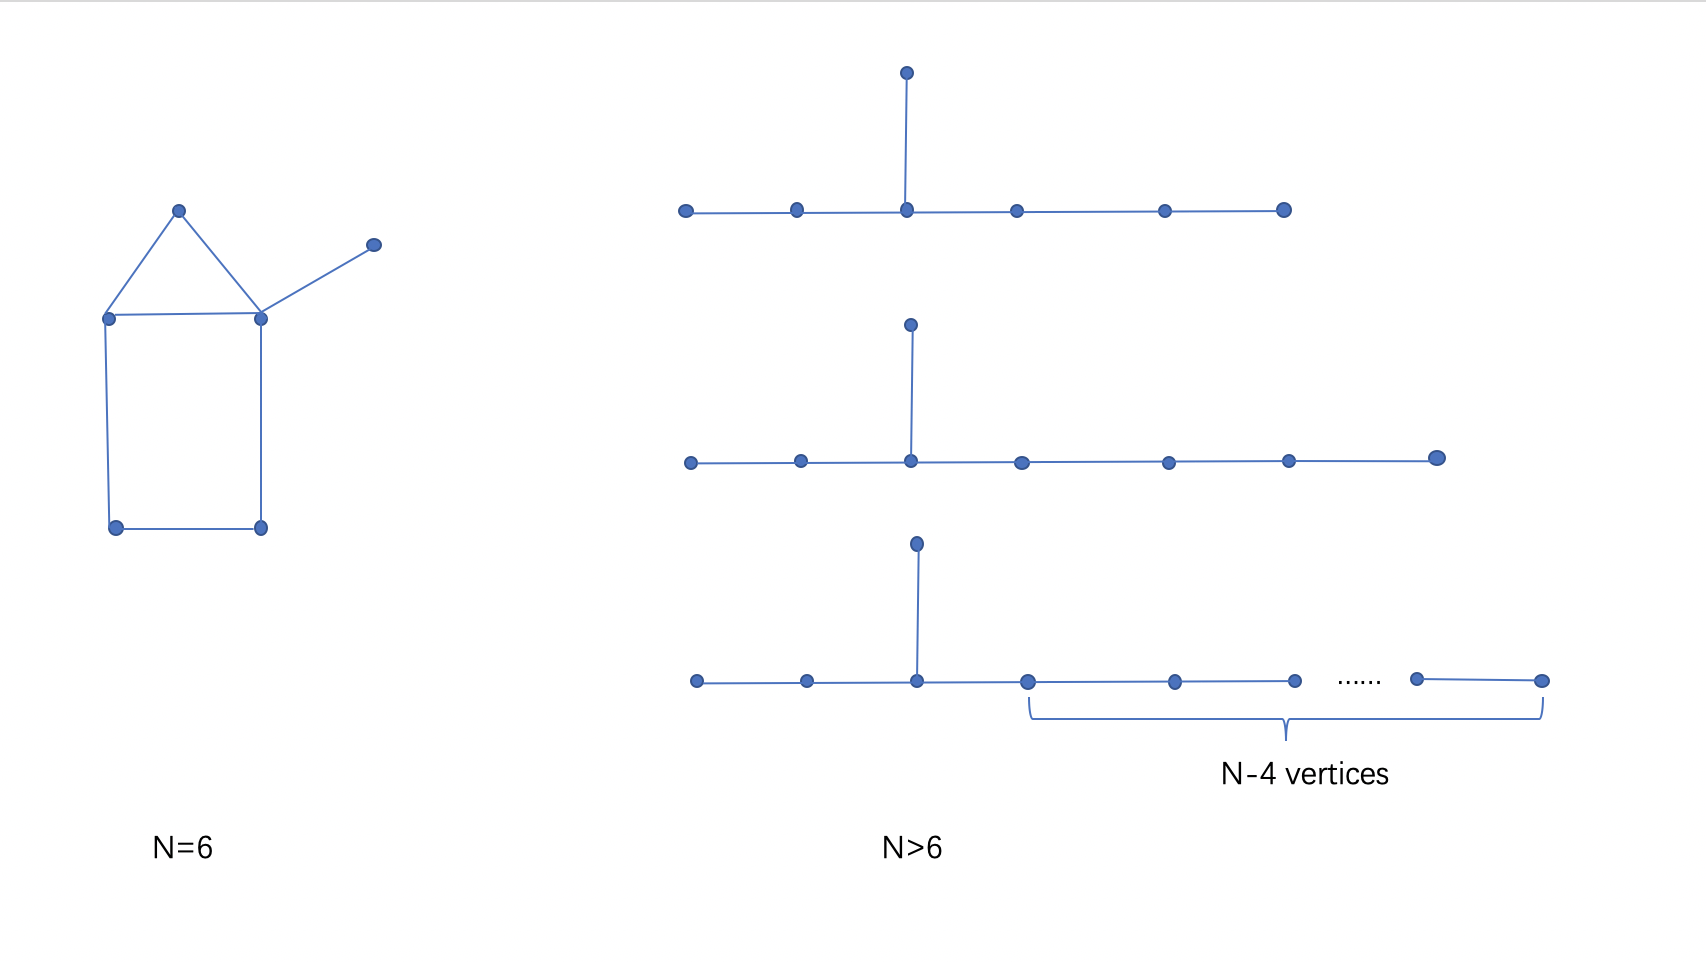
\includegraphics[scale=0.4]{65.png}
  	\caption{}
  	\label{fig:6}
  	\end{figure}
	When $n=6$, the left graph is correct. When $n>6$, we just need to construct trees like right graphs. 
	There are only one vertex that has three degrees and  $n-4$ vertices are at the right of this vertex.
	 
	\textbf{Exercise 6.6}\par
	For graphs in \textbf{Exercise 6.5}, we just need to add cherries for every vertex, like Figure $2$.
	\begin{figure}[H]
  	\centering
  	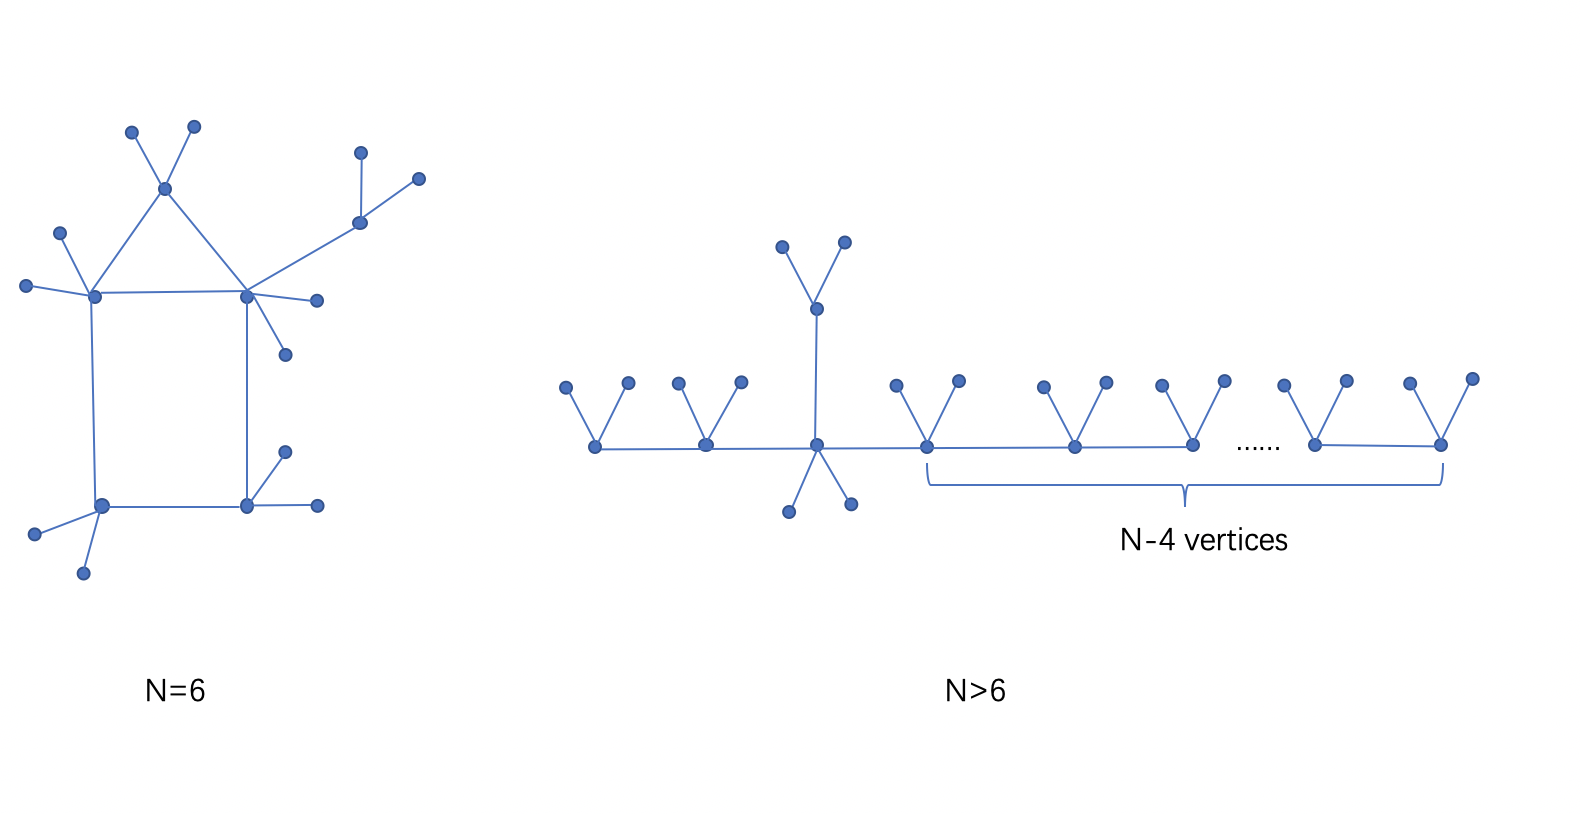
\includegraphics[scale=0.4]{66.png}
  	\caption{}
  	\label{fig:7}
  	\end{figure}
	The graph has $3n$ vertices with $2^{n}$ automorphisms.\par
	
	\textbf{Exercise 6.7}\par
	\textbf{1.} We can use $4p+1$ to form such graph with the method showed in \textbf{Exercise 6.4}\par
	\textbf{2.} There is no such graph with less than $p$ vertexes. \par
	As the conclusion we got from class goes, for a graph with p vertexes, the number of its automorphisms can divide $p!$. Any prime number bigger than $p$ cannot divide $p!$, so There is no such graph with less than $p$ vertexes. \par

	
	\textbf{Question:}\par
	In Exercise 6.7, if we do not include the constraint that P is a prime number, what conclusion can we get? First, we make a prime factorization on P, which is $P=P_1^{A_1}\cdot P_2^{A_2}\cdot \cdots \cdot P_n^{A_n}$
  	For every i, $P_i$ is prime number and $A_i$ is positive integer.
	We have a hypothesis that the number of vertices might be $O(P_{max}+A_{max})$. But we don’t know how to prove it. Or do we have another answer?


\end{document}
	

